%%%%%%%%%%%%%%%%%%%%%%%%%%%%%%%%%%%%%
\chapter{Standard Model and rare Z and Higgs decays to quarkonia}
\label{chaptertheory}

\section{Standard Model and Local Gauge Invariance}
\label{section_sm}

% The human quest for understanding the Universe, goes through taking a complex problem and break it down into smaller (simpler) ideas, that, when stacked together, gives rise to a proper explanation of a phenomenon and, in the best scenario, allows us to make predictions about unexpected or less known aspects of subject. The Standard Model (SM) embodies this idea and attempts not only to explain the Universe in fundamental process (interactions), but also in terms of fundamentals components (particles). To what it proposes to explain, the Standard Model have been proven very effective.
 
Physics understands matter and how it interacts in terms of two components: fundamentals forces and elementary particles. From the weakest to the strongest, the fundamental forces are: Gravitational, Weak, Electromagnetic and Strong. All share common characteristics like, being mediated by particles~\footnote{There is no evidence of the existence of the Graviton (force carrier associated to the gravitational force), even though, it is theorized by models that wish to comprehend gravity in a quantum perspective.}, being relevant within some effective range and have a associate a charge-like quantity (i.e. an intrinsic characteristic of the object) that defines whether or not, particles might be subjected to a specific interaction.

Along with the fundamental interactions, the Standard Model~\cite{burgess_moore_2006, oguri_qcd, Halzen:1984mc, Aitchison:2004cs} (or simply \textit{SM}) defines every existing matter in the Universe as a set of fundamental quantum objects, with properties that prescribes their interaction. Those objects are said to be fundamental since, in the context of the SM, they are the smallest possible components of matter. We shall refer to them as \textit{Fundamental Particles}. There four of those mediating particles (force carriers), gluon ($g$ - for the strong interaction), photon ($\gamma$ - for the electromagnetic interaction), Z (neutral) and $W^\pm$ (for weak interaction), all of them being vector bosons (spin 1). Besides the interaction mediators, described at Table~\ref{fundamental_forces}, the fundamental particles are divided in two groups (\textit{quarks} and \textit{leptons}), with three generations, each. These are not force carriers, but elementary particles, endowed with charge-like characteristics that allow them to interact by exchange the vector bosons. Those are the building blocks of Matter in our Universe.

Figure~\ref{sm_summary} summarizes their properties. Table~\ref{fundamental_forces} presents the relative strength and effective range, for each on of the four fundamental interactions. It is important to stress that, the gravitational force is not study subject of the Standard Model.

\begin{figure}[!htbp]
  \begin{center}
  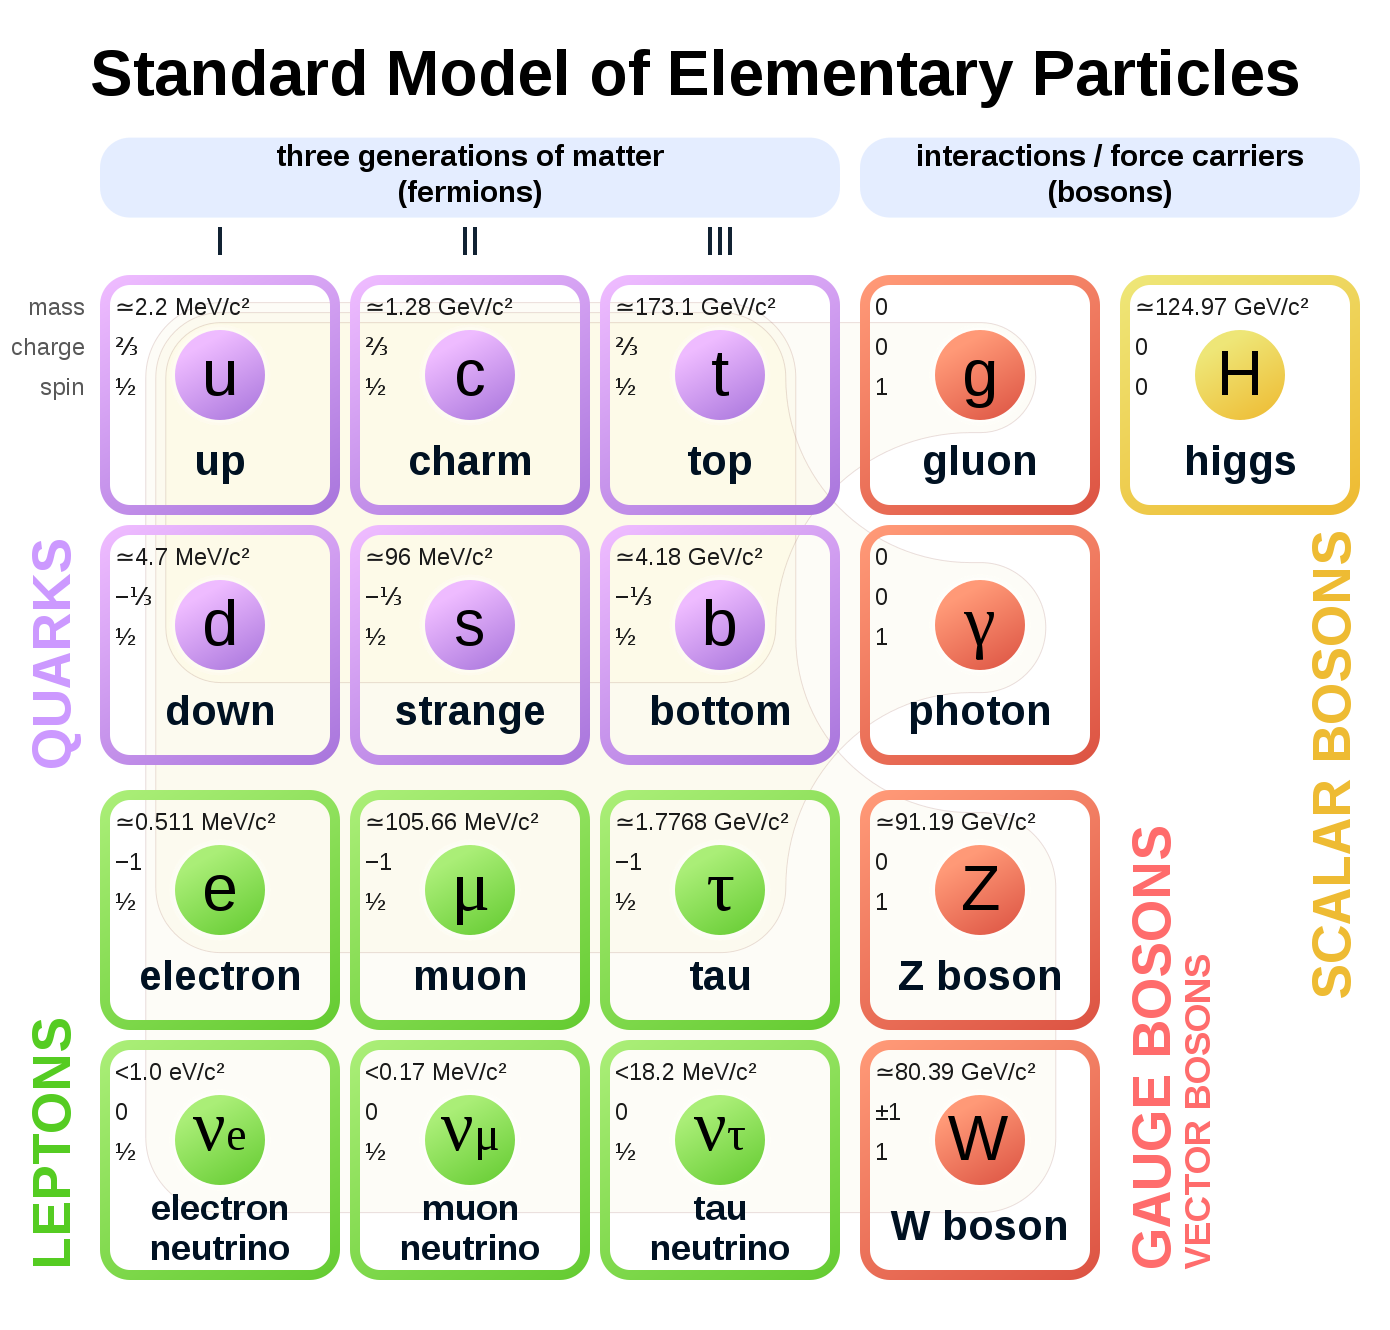
\includegraphics[width=0.6\textwidth ]{figures_and_tables/theory/sm.png}
  \end{center}\vspace*{-.5cm}
  \caption{Elementary particles of the Standard Model, with their masses charges and spin. Those particles can be divided in two classes: boson (the interaction/force carriers) and the fermions, which are divided in three generations. Source:~\cite{fig_sm_summary}.}
  \label{sm_summary}
  \end{figure}
 

\begin{table}[htp]
  \begin{center}
      \caption{Relative strength (with respect to the strong force) and effective range of action for the four fundamentals interactions.}
    \begin{tabular}{ cccc }
       & Mediator & Relative Strength & Effective Range \\ \hline
      Gravitational & Graviton & $10^{-41}$ & $\infty$ \\ 
      Weak & W and Z & $10^{-16}$ & $10^{-18}$ m \\ 
      Electromagnetic & Photon & $10^{-3}$ & $\infty$ \\ 
      Strong & Gluon & $1$ & $10^{-15}$ m\\ \hline
      \end{tabular}
  \label{fundamental_forces}
  \end{center} 
  \end{table}


There are six quarks, up and down ($u$ and $d$ - first generation), charm and strange ($c$ and $s$ - second generation), top and bottom ($t$ and $b$ - third generation), in increasing invariant mass order of the generations. Since they interact through all the three fundamental forces of the SM, they are said to possess electrical charge (for the electromagnetic interaction), flavour (for the weak interaction) and color (for the strong). Their generational counterparts, the leptons, don't interact via strong force, that is why they are said to have only flavour and electric charge. The leptons are electron and electron neutrino ($e$ and $\nu_e$ - first generation), muon and muon neutrino ($\mu$ and $\nu_{\mu}$ - second generation) and tau and tau neutrino ($\tau$ and $\nu_{\tau}$ - third generation). The neutrinos, within the SM, are massless, even though, experimental measurements have shown that they actually have mass~\cite{pdg_2020}. Neutrinos are also electrically neutral, meaning that they only interact through weak interactions.

Figure~\ref{sm_summary} also presents the Higgs Boson ($H$) which is part of the SM and shall be discussed later.

\subsection{Local Gauge Invariance}
\label{lgi_qed}

Within the Standard Model, the theoretical basis that describe the fundamental interactions are derived from a common principle: the local gauge invariance. According to Salam and Ward~\cite{ward_salam}:

\begin{quote}
  "Our basic postulate is that it should be possible to generate strong, weak and electro-magnetic interaction terms [...], by making local gauge transformations on the kinetic-energy terms in the free Lagrangian for all particles."
\end{quote}

Taking the Quantum Electrodynamics (QED) as an example: the quantum field theory that describes the electromagnetic interactions, consider the Dirac equation, in the covariant form, for a particle with mass $m$, charge $-e$ and spin $1/2$, i.e. a electron:

\begin{equation}
    (i \gamma^\mu \partial_\mu + m)\psi(x) = 0,
    \label{dirac_equation}
\end{equation}
where $\psi(x)$ is a spinor, describing the wave-function and $\gamma^\mu$ are gamma-matrices. This equation can be obtained from the lagrangian $\mathcal{L}$~\footnote{Even though, the $\mathcal{L}$ actually represents the lagrangian density, in this document we shall refer to it as simply lagrangian.} of a free particle, in the form of 

\begin{equation}
    \mathcal{L_{\text{0}}} = i\bar{\psi}(x)\gamma^\mu\partial_\mu\psi(x)-m\bar{\psi}\psi(x),
    \label{lagrangian_free_particle}
\end{equation}
when applied to the Euler-Lagrange equation.

It is clear that, the Dirac Equation (\ref{dirac_equation}) and its lagrangian (\ref{lagrangian_free_particle}) are invariant under a global phase transformation.

\begin{equation}
    \psi(x) \rightarrow \psi'(x) = \exp{(-ie\alpha)}\psi(x),
    \label{global_phase_transformation}
\end{equation}
where is a constant (global phase shift).

The same is not true when $\alpha$ is not a constant, but actually a local phase transformation, a gauge transform.

\begin{equation}
    \psi(x) \rightarrow \psi'(x) = \exp{(-ie\alpha(x))}\psi(x)
    \label{local_phase_transformation}
\end{equation}

In this case, the derivative of $\alpha(x)$ will introduce a new term that would break the invariance. To recover it, the covariant derivative operator should be modified as follows:

\begin{equation}
    \partial_\mu \rightarrow D_\mu = \partial_\mu - ieA_\mu.
    \label{covariant_derivative_modification}
\end{equation}

This modification introduces the concept of the gauge field $A_\mu$, associated to a particle of spin 1 and zero mass, the photon. This term should transform under gauge, in the following manner:

\begin{equation}
    A_\mu \rightarrow A'_\mu = A_\mu - \partial_\mu\alpha(x).
    \label{covariant_gauge_field}
\end{equation}

Modifications \ref{covariant_derivative_modification} and \ref{covariant_gauge_field} are sufficient not only to make the free particle Dirac Equation and its lagrangian gauge transformation invariant (Equations \ref{invariant_dirac_equation} and \ref{invariant_lagrangian} ), but also it naturally gives rise to an interaction term associated to the gauge field $A_\mu$.

\begin{equation}
        (i \gamma^\mu \partial_\mu + m)\psi(x) = -e\gamma_\mu A_\mu(x) \psi(x) 
    \label{invariant_dirac_equation}
\end{equation}
\begin{equation}
    \begin{split}
        \mathcal{L} \rightarrow \mathcal{L'} &= i\bar{\psi'}(x)\gamma^\mu\ D_\mu\psi'(x)-m\bar{\psi'}\psi'(x) \\
        \mathcal{L'} &= \mathcal{L_{\text{0}}} + e\bar{\psi}(x)\gamma^\mu A_\mu \psi(x) = \mathcal{L}
    \end{split}
    \label{invariant_lagrangian}
\end{equation}

Interesting to notice that the $\mathcal{L_{\text{0}}}$ term, on \ref{invariant_lagrangian}, corresponds to the electron kinetic energy plus its mass contribution (the free particle lagrangian), while the second corresponds to the interaction of the electron ($\psi(x)$) and the electromagnetic field. On this basis, $e$ is said to be the generator of the electromagnetic four-potential, $A_\mu$. One could add the energy contribution of the electromagnetic field itself, by adding a term like:

\begin{equation}
    \mathcal{L_{\text{EM}}} = - \frac{1}{4} F_{\mu\nu} F^{\mu\nu},
\label{lagragian_em}
\end{equation}
where:
\begin{equation}
    F_{\mu\nu} = \partial_\mu A_\nu - \partial_\nu A_\mu
\label{f_munu_definition}
\end{equation}
is the electromagnetic field tensor.

It can be proven that applying \ref{f_munu_definition} on the Euler-Lagrange equations, this will give us the Maxwell's Equations for the vacuum, $\partial_{\mu} F^{\mu\nu} = 0$~\footnote{A non-vacuum covariant form of the Maxwell's Equations would be $\partial_{\mu} F^{\mu\nu} = j^{\nu}$.}. One could also expect that a field mass contribution in as below, could be introduced, as well.

\begin{equation}
    \frac{1}{2}m_{photon}^2 A_\mu A^\mu
\label{photon_mass_term}
\end{equation}

This one would break the gauge invariance, therefore we can imply that the photon should be massless.

The QED is said to be a gauge theory with the symmetry group $U(1)$. The $U(1)$ description comes from Lie Algebra, where \ref{covariant_derivative_modification} and \ref{covariant_gauge_field} are transformations of gauge $\alpha$ (in one dimension) to which the system is symmetric (invariant), then unitary and generated by a $1 \times 1$ matrix ($e$).

\subsection{The Standard Model}

Taking profit of the Local Gauge Invariance as path to introduce interactions in a quantum field theory (QFT), such as for the QED, the Standard Model can be defined as a QFT of the gauge group $SU_{\scaleto{c}{5pt}}(3) \times SU_{\scaleto{L}{5pt}}(2) \times U_{\scaleto{Y}{5pt}}(1)$. All the experimental results we have, so far (Section~\ref{section_sm_higgs_results}), give us support to this definition. 

In this context there are 8 spin 1 bosons (called gluons) for the $SU_{\scaleto{c}{5pt}}(3)$ component, which corresponds to the strong interaction, plus 4 bosons, $W^\pm$, $Z$ and the photon for the other components (weak and electromagnetic interactions).

Hadrons are defined as colorless particles that interact strongly. They are bound states of quarks, which also interact via strong force and have non-neutral color. Hadrons are divided in mesons (spin integer) and barions (spin non-integer). Leptons are those particles that do not interact via gluons.

\subsubsection{Quantum Chromodinamics}

Quantum Chromodynamics (QCD) is the $SU_{\scaleto{c}{5pt}}(3)$ component of the SM, where $SU$ stands for special unitary group, to which the $det(e^{i\lambda_i}) = 1$, where $\lambda_i$ are the Gell-Mann matrices (the 8 generators of the $SU(3)$). It corresponds to the field of gluons, responsible for the strong interaction acting on a charge-like degree of freedom: colour ($c$). Gluons follow the same fashion as photons, they are massless and have spin 1, but contrary to electromagnetism, the QCD is a non-abelian gauge theory. This means that the force carriers (gluons) can interact with each other (self-coupling). In other words, gluons are charged (coloured). In a more formal manner, the generators of this group are non-commutative, as follows.

\begin{equation}
    \left[ T_a, T_b \right] = \left[ \frac{\lambda_a}{2}, \frac{\lambda_b}{2} \right] = i \sum_{c=1}^8 f_{ab}^c\lambda_c,
\label{qcd_commutators}
\end{equation}
where $f_{ab}^c$ are antisymmetric structure constants.

From a experimental perspective, the idea of colour begins with the observation of $\Lambda^{++}$~\cite{dalitz1967proceedings}. It could be only be composed by three up quarks, which would break Pauli Exclusion Principle~\footnote{Two or more fermion can not be in the same quantum state.}. This observation demanded the inclusion of another degree of freedom, the colour, typically refereed as RED, BLUE, GREEN and its anti-colours.

The QCD lagrangian for a quark of colour $c$, just the QED lagrangian for a electron of charge $-e$, is~\footnote{The total QD lagrangian would the sum over all possible states.}:

\begin{equation}
    \mathcal{L_{QCD}} = \bar{\psi_c}(x)(i\gamma^\mu\ D_\mu -m)\psi_c(x) - \frac{G_{\mu\nu}^c G^{\mu\nu}_c}{4},
\label{qcd_lagrangian}
\end{equation}
where
\begin{equation}
    D_\mu = \partial_\mu + ig_s T_c G_\mu^c
\label{qcd_lagrangian_definitions1}
\end{equation}
and 
\begin{equation}
    G_{\mu\nu}^c = \partial_\mu G_\nu^c - \partial_\nu G_\mu^c - g_s f_{ab}^c G_\mu^a G_\nu^b
\label{qcd_lagrangian_definitions2}
\end{equation}

This lagrangian is local gauge invariant when the strength tensor \ref{qcd_lagrangian_definitions2} as:

\begin{equation}
    G_{\mu}^c \rightarrow {G_{\mu}^c}' = G_{\mu}^c - \frac{1}{g_s} \partial_\mu \alpha_c(x) - f_{ab}^c \alpha_a(x) G_{\mu}^b
\label{strength_tensor_tranform}
\end{equation}

Coloured particles, such as quarks and gluons, are subjected to the phenomenon of Colour Confinement, which prohibits the direct observation of these particles. These can only be observed in colourless bound states (hadrons). A isolated quark or gluon will immediately interact with the vacuum and initiates a hadronization process until a set of stable colourless particle is produced. As a consequence of the Colour Confinement and the self-coupling property of gluons, a bound state of gluons, Glueballs~\cite{wolfgang_status}, is possible, even though there are no experimental clear evidences of its existence. This is one of the few open topics in the SM.

QCD is a perturbation theory ($\mathcal{L} = \mathcal{L}_{\text{Free Particle}} + \mathcal{L}_{\text{Interaction}}$) which demands renormalization~\footnote{A techniques to deal with infinites that might arrive when calculating quantities in a QFT. In summary the total probability for the theory is required to re-sum to unity.}. In a qualitative way, one could imagine that, as larger the distance on interaction is, more sea vacuum gluon pairs can contribute to the net colour charge, due to the self-coupling, increasing the total interaction strength. To cope the Colour Confinement and the self-coupling, one would redefine the the strong coupling constant as $g_s = \sqrt{4 \pi \alpha_s}$ (from \ref{qcd_lagrangian_definitions1}, \ref{qcd_lagrangian_definitions2} and \ref{strength_tensor_tranform}), where $\alpha_s(Q^2) \propto \frac{\Lambda^2_{QCD}}{ln Q^2}$. In this situation, the coupling strength is related to the transferred momentum $Q^2$, in such a way that, in a highly energetic interaction (high $Q^2$, hence short distance) the coupling is weaker and the quarks and gluons involved, behave like a quasi-free particles, allowing the use of perturbation theory. This effect is known as Asymptotic Freedom, and its scale have already been measured by the LHC experiments~\cite{pdg_2020}.

\subsubsection{Electroweak Theory}

The $SU_{\scaleto{L}{5pt}}(2) \times U_{\scaleto{Y}{5pt}}(1)$ represents the Electroweak component of the SM. It is the unification of the Weak and Electromagnet interaction, under the same theory. Here two new degrees of freedom are introduced, $L$ and $Y$. The former one is related to the chirality of $SU(2)$ and the latter is the weak hypercharge. The generators of groups are the Pauli Matrices ($T_i$)~\footnote{The usual $\sigma_i$ representation for the Pauli Matrices usually is reserved for the $SU_{\scaleto{spin}{5pt}}(2)$ group.}, form the $SU_{\scaleto{L}{5pt}}(2)$ and the electromagnetic generator structure for $U_{\scaleto{Y}{5pt}}(1)$ (but for $Y$, instead of $-e$, as before). Since:

\begin{equation}
    \begin{split}
        \left[ T_a, T_b \right] &=  i \levicivita{^{abc}}T_c,  \\
        \left[ T_a, Y \right] &=  0
    \end{split}
\label{pauli_commutator}
\end{equation}
where $\levicivita{^{abc}}$ is the Levi-Civita tensor, $SU_{\scaleto{L}{5pt}}(2)$ is also a non-abelian group.

The connection between electric charge $Q$ and the weak charge is $\frac{Y}{2} = Q - T_3$, as such, QED ($U_{\scaleto{EM}{5pt}}(1)$), as defined in Section~\ref{lgi_qed} is derived from $U_{\scaleto{Y}{5pt}}(1)$.

In the Electroweak Theory, fermions can have left-handed or right-handed components of their wave-functions, according to their chirality. Left-handed components transform as doublets of $(T, T_3)$ with eigenvalues $(1/2, \pm1/2)$ under $SU_{\scaleto{L}{5pt}}(2)$ and the right-handed components transform as singlets $(T=0)$. Weak interactions act only on left-handed fermions. That is the reason for the $L$ subscript in the electroweak symmetry group definition.

\subsubsection{Standard Model Lagrangian and the Higgs Sector}

The SM lagrangian is given by:
\begin{equation}
        \mathcal{L}_{SM} =  \mathcal{L}_{gauge} + \mathcal{L}_{fermions} + \mathcal{L}_{Yukawa} + \mathcal{L}_{Higgs},
\label{sm_lagrangian}
\end{equation}
where $\mathcal{L}_{gauge}$ describes gauge fields of the QCD and Electroweak theories,

\begin{equation}
    \mathcal{L}_{gauge} =  -\frac{1}{4}\sum_{c = 1}^{8}G_{\mu\nu}^c G^{\mu\nu}_c -\frac{1}{4}\sum_{a = 1}^{3}W_{\mu\nu}^a W^{\mu\nu}_a  -\frac{1}{4}B_{\mu\nu} B^{\mu\nu} .
\label{sm_lagrangian_gauge}
\end{equation} 

The first term is related to the $SU_{\scaleto{c}{5pt}}(3)$ component of the SM and last two terms are related to $SU_{\scaleto{L}{5pt}}(2) \times U_{\scaleto{Y}{5pt}}(1)$ components, respectively. The summations are related to all generators in the symmetry group, $8$ and $3 + 1$, for QCD Electroweak.  Following the same structure as in \ref{qcd_lagrangian_definitions2}:

\begin{equation}
    \begin{split}
        W_{\mu\nu}^a &= \partial_\mu W_\nu^a - \partial_\nu W_\mu^a - g \levicivita{_{abc}} W_\mu^b W_\nu^c,  \\
        B_{\mu\nu} &= \partial_\mu B_\nu - \partial_\nu B_\mu
    \end{split}
\label{electroweak_field}
\end{equation}


For the fermionic term of the lagrangian, we have:
\begin{equation}
    \mathcal{L}_{fermions} = \sum_j i \bar{\psi}_L^j \slashed{D}^L \psi_L^j + \sum_k i \bar{\psi}_R^k \slashed{D}^R \psi_R^k,
\label{sm_lagrangian_fermionic}
\end{equation} 
where the first term is summed over all $T$ doublets (left-handed components) and the second one, over all $T$ singlets (right-handed components). The slash notation was introduced, in which $\slashed{a} = \gamma^\mu a_\mu$. Here, we define the covariant derivatives as:

\begin{equation}
    \begin{split}
        D_\mu^L &= \partial_\mu + ig \sum^3_{a=1} T_L^a W_\mu^a + ig'\frac{Y}{2}B_\mu + ig_sT_cG_\mu^c  \\
        D_\mu^R &= \partial_\mu + ig'\frac{Y}{2}B_\mu + ig_sT_cG_\mu^c 
    \end{split}
\label{electroweak_invariant_derivative}
\end{equation}

It is important to notice that, the weak interaction term ($W_\mu$) is absent in the right-handed component and the QCD term of the covariant derivative is only applied to quarks. Leptons are colourless.

Since, the electroweak components of the SM are not related to flavour and charge, but rather weak hypercharge and left-handed chirality, the boson that we observe experimentally ($Z$, $W^\pm$ and $\gamma$) are not directly related to the fields $W_\mu^a$ and $B_\mu$. They are linear combination of them, as follows (assuming $T_L^a = \sigma^a/2$, where $\sigma^a$ are the Pauli Matrices):

\begin{equation}
    W^{\pm}_\mu = \frac{1}{\sqrt{2}} W_\mu^1 \mp i W_\mu^2
\label{eletroweak_linear_combinations_W}
\end{equation}
\begin{equation}
    \begin{split}
        Z_\mu &= cos \theta_w W^3_\mu - sin \theta_w B_\mu, \\
        A_\mu &= sin \theta_w W^3_\mu + cos \theta_w B_\mu,
    \end{split}
\label{eletroweak_linear_combinations_z_gamma}
\end{equation}
where $\theta_w$ is a measurable of the theory~\cite{pdg_2020}.


The SM lagrangian terms, presented so far, are clearly gauge invariant, under the proper transformations. Even though this is sufficient to define the interactions, two problems arise, related to mass: the spin 1 gauge boson are, by construction, massless, which is in conflict for the measurements we have for $Z$ and $W^\pm$~\cite{pdg_2020}; if one include a mass term for the fermions, as expected from the previous discussion on the QED and QCD, this would break the gauge invariance of the symmetry.

The overcome these problem, another field ($\phi$) is introduced. By its interaction with Electroweak bosons ($Z$ and $W^\pm$), they gain mass. Also, at the same time, a Yukawa coupling term, between the new field and the fermion, is capable to give them mass, naturally. The simplest way to achieve this is by introducing a scalar field double in $SU_{\scaleto{L}{5pt}}(2)$, the Higgs field.

\begin{equation}
    \phi = 
        \left ( 
        \begin{matrix}
        \phi^+ \\
        \phi^0 
        \end{matrix}
        \right )
    \label{higgs_field}
\end{equation}

Therefore, the Higgs contribution to the SM lagrangian is:

\begin{equation}
    \mathcal{L}_{Higgs} = (D_\mu\phi)^\dagger(D_\mu\phi) - V(\phi),
    \label{higgs_field1}
\end{equation}
where
\begin{equation}
    D_\mu = \partial^\mu + ig \sum^3_{a=1} T_L^a W_\mu^a + ig'\frac{Y}{2}B_\mu
    \label{higgs_field2}
\end{equation}
and 
\begin{equation}
    V(\phi) = \mu^2 \phi^\dagger \phi + \lambda(\phi^\dagger \phi)^2.
    \label{higgs_field3}
\end{equation}

The key idea behind the introduction of this field, is that, at ground state, the $SU_{\scaleto{L}{5pt}}(3) \times U_{\scaleto{Y}{5pt}}(1)$ symmetry is "spontaneously" broken, hence the name usually given to this procedure Spontaneously Symmetry Break~\cite{Higgs:1964pj, Higgs:1964ia, Higgs:1966ev, Englert:1964et, Guralnik:1964eu, Kibble:1967sv}. In this case, to preserve unitarity and to ensure the $V(\phi)$ has a global minimum, $\lambda > 0$.  and $\mu^2$ needs to be negative, in order to give mass to $Z$ and $W^\pm$, otherwise, we would be adding just a scalar field of mass $\mu$ with self-coupling of strength $\lambda$, but the SM bosons would still be massless.

In this case, the minimum value for $V(\phi)$ is a set of degenerated states in a circle of radius $<\phi> = \sqrt{\frac{-\mu^2}{2\lambda}} = \frac{v}{\sqrt{2}}$, $v = \sqrt{-\mu^2/\lambda}$ is the vacuum expectation value (VEV). Without loss of generality, one can choose a direction:

\begin{equation}
    \phi = \frac{1}{\sqrt{2}}
        \left ( 
        \begin{matrix}
        0 \\
        v 
        \end{matrix}
        \right )
    \label{higgs_field_vev_based}
\end{equation}
assigning hypercharge $Y=1$.

Once again, taking profit of the perturbation theory around the ground state (VEV), one could define~\footnote{A even more general redefinition of the Higgs field would be possible ($\phi = (\phi^+, v + H +i \chi)$), but the one proposed presents no loss of generality.}:

\begin{equation}
    \phi = \frac{1}{\sqrt{2}}
        \left ( 
        \begin{matrix}
        0 \\
        v + H
        \end{matrix}
        \right )
    \label{higgs_field_vev_based}
\end{equation}

Expanding the potential $V(\phi)$, as is \ref{higgs_field3}, one gets:

\begin{equation}
    V = \mu^2 H^2 + \frac{\mu^2}{v} H^3 + \frac{\mu^2}{4v^2} H^4,
    \label{higgs_mass_term}
\end{equation}
hence, a new scalar boson (the Higgs boson) is included in the the theory with mass $\sqrt{2\mu^2}$ and self-couplings terms.

In the same way, expanding \ref{higgs_field2} and assuming $T_L^a = \sigma^a/2$: 
\begin{equation}
    (D_\mu\phi)^\dagger(D_\mu\phi) = \frac{1}{2}(\partial_\mu H)^2 + \frac{1}{8}g^2(v+H)^2|W_\mu^1+iW_\mu^2|^2 + \frac{1}{8}(v+H)^2|gW_\mu^3-g'B_\mu|^2.
    \label{higgs_mass_term}
\end{equation}

Defining the SM bosons fields as:

\begin{equation}
    \begin{split}
        W_\mu^\pm &= \frac{1}{\sqrt{2}} (W_\mu^1 \mp iW_\mu^2) \\ 
        Z_\mu &= \frac{gW_\mu^3-g'B_\mu}{\sqrt{g^2+g'^2}} \\ 
        A_\mu &= \frac{gW_\mu^3+g'B_\mu}{\sqrt{g^2+g'^2}},
    \end{split}
    \label{sm_bosons_fields}
\end{equation}
one can naturally infer that the introduction of the Higgs fields gave the SM bosons mass values of: $M_W = vg/2$, $M_Z = v\sqrt(g^2+g'^2)$ and $M_A = 0$. In this context, the Weinberg angle, $\theta_W$, is related to the SM coupling constants as:

\begin{equation}
    \begin{split}
        cos \theta_W = \frac{g'}{\sqrt{g^2+g'^2}} \\ 
        sin \theta_W = \frac{g}{\sqrt{g^2+g'^2}}.
    \end{split}
    \label{weinberg_angles}
\end{equation}

The missing piece of the SM lagragian (\ref{sm_lagrangian}) is the Yukawa components, $\mathcal{L}_{Yukawa}$, and how it gives the fermion masses. The procedure is quite straightforward. Start including a Yukawa coupling for each fermion to either $\phi$ or $\tilde{\phi} =i \sigma_2 \phi^\dagger$ (this one with $Y=-1$). Taking the electron as an example:

\begin{equation}
    \begin{split}
        \mathcal{L}_{Yuk}^e &= -\lambda_e \bar{L} \phi e_R + h.c. \\
        \mathcal{L}_{Yuk}^e &= -\frac{1}{\sqrt{2}} \lambda_e (\bar{\nu^e}, \bar{e_L}) \left ( 
            \begin{matrix}
            0 \\
            v + H
            \end{matrix}
            \right )
            e_R + h.c \\ 
        \mathcal{L}_{Yuk}^e &= -\frac{1}{\sqrt{2}} \lambda_e  (v+H) \bar{e}_Le_R + h.c,
    \end{split}
    \label{fermion_mass}
\end{equation}
where $\lambda_e$ is the coupling constant between the Higgs boson and the electron. This tell us that $m_e = \frac{\lambda_e v}{\sqrt{2}}$.

Similar procedure can be used for all the fermion of the SM. 
